\documentclass[12pt,a4paper]{scrartcl}

\usepackage[T1]{fontenc}
\usepackage[utf8]{inputenc}
\usepackage[magyar]{babel}
\usepackage{lmodern}
%% Sets page size and margins
\usepackage[a4paper,top=3cm,bottom=2cm,left=3cm,right=3cm,marginparwidth=1.75cm]{geometry}

\usepackage{graphicx}
\usepackage{amsmath}
\usepackage{amsfonts}
\usepackage{amssymb}
\usepackage{bm}
\let\mathbf\bm

\usepackage{placeins}
\usepackage{subcaption}
\usepackage{epstopdf}
\usepackage{xcolor}
\usepackage[hidelinks,unicode]{hyperref}
\hypersetup{
    colorlinks,
    linkcolor={red!50!black},
    citecolor={blue!50!black},
    urlcolor={blue!80!black}
}

\usepackage{cleveref}

\title{Felületi feszültség\\{\small{7. tétel}}}
\author{Tüzes Dániel}
\date{\today}
\begin{document}
\maketitle

\section{Felületi feszültség}
A felületi feszültség nyugvó gáz és folyadék, illetve szilárd anyagra bevezetett fogalom, ahol két különféle halmazállapotú anyag (akár azonos halmazállapotból véve) közötti határfelületet vizsgáljuk. Általában nem vizsgálunk szilárd anyag-szilárd anyag határfelületet, mert közöttük a feszültségtenzor nyíró komponenst is tartalmazhat, tehát azok az egységmátrixnak nem skalárszorosai, így esetükben nyomásról nem beszélhetünk.

\footnotesize
\paragraph{Demonstráció} Egy vékony pengét a víz felszínére teszünk. A penge sűrűsége nagyobb, mint a vízé, alakja nem konkáv, így a víz nem tud akkora felhajtóerőt kifejteni rá, ami meggátolhatná az elsüllyedésben. Mégis, a víz felszínére óvatosan ráhelyezett penge nem merül el a vízben. Ha a víz alá nyomjuk, akkor már elsüllyed.

A víz felszínén úszó, lemezből készült hajókának a végére étert cseppentünk, akkor a hajó elindul előre. Szappan bekenve a végét hasonló jelenséget tapasztalunk.

Egy pohár tetejét egy rétegben egy hálóval fedjük be, pl.\ gézlappal. A poharat megtöltjük vízzel. Ha a poharat ügyesen megfordítjuk, akkor a víz nem jön ki a pohárból, annak ellenére, hogy a hálón könnyen át tudna folyni. Ha a hálóhoz hozzáérünk, a folyadék kifolyik.
\normalsize

Megfigyelés: Ha egy téglalap drótkeretén szappanhártya feszül, és a téglalap egyik oldala szabadon mozoghat, akkor a szappanhártya a szabadon mozgó oldalt elmozdítja úgy, hogy a téglalap területe csökkenjen. Ahhoz, hogy a szabad oldal ne mozduljon el, erőt kell kifejteni, aminek a nagysága függ az anyagi minőségtől, és a keretben lévő szál hosszától.
\[F = 2\alpha  \cdot l\]
A definícióban szereplő $2$-es nem véletlen, bár egyelőre csak definíció kérdése a léte. Ebben a képletben $\alpha$-t felületi feszültségnek nevezzük, és a  mértékegysége $\text{ N}/\text{m}$.

\begin{figure}[htbp]
	\begin{center}
		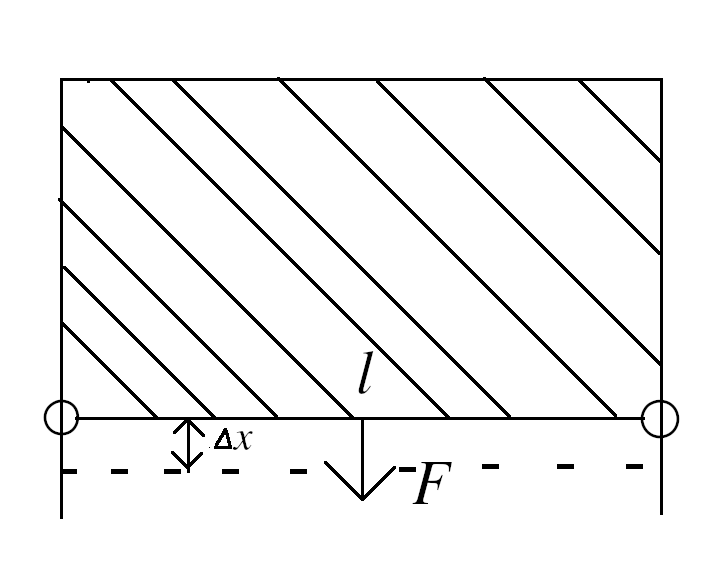
\includegraphics[width=0.4\textwidth]{tetel7.png}
		\caption{A fémkeret, benne a hártyával. $F$ erővel $\Delta x$ távolsággal kihúzzuk, így a felület $\Delta A =  2l \cdot \Delta x$-nyit megnő. A kettes szorzó azt fejezi ki, hogy a felületnek két oldala van.}
	\end{center}
\end{figure}

A felületi feszültségnek egy másik értelmezését is megadhatjuk, ha feltesszük a kérdést, hogy mennyivel változik meg a hártya által tárolt energia, miközben megváltoztatom a hártya nagyságát? Ehhez keret oldalát mozdítsuk el egy $\Delta x$ távolsággal! A mozgatás során erő nem változik, így a végzett munka
\[\Delta W = F \cdot \Delta x = \alpha 2l \cdot \Delta x = \alpha  \cdot \Delta A.\]

A felületi feszültségre ebből a képletből adódik az alábbi alak:
\[\alpha  = \frac{{dW}}{{dA}}.\]

Ha a felületi feszültség definíciójának ezt tekintjük, akkor ebben már nincs 2-es, és amúgy pontosan ezért lett korábban az erő kifejezésében egy 2-es beleépítve, hogy ebben már ne legyen. A felületi feszültség tehát megadja, hogy mennyivel nő meg egy felület energiája, ha a felszínét megváltoztatom.

A felületi feszültség minden határfelületen fellép. Energetikai szempontból a minimális határfelületű alakzatok a legkedvezőbbek, ezért a hártya mindig abba az alakba igyekszik beállni. 

\footnotesize
\paragraph{Demonstráció} Egy 2D-s keret esetén, ha a keret alakja téglalap, triviális, hogy mi a minimális felület, ha az egyik oldalt szabadon mozgathatjuk. Nem triviális azonban, ha a peremfeltételeket 3D-ben írjuk fel. A megoldásokat egyből láthatjuk, amennyiben a peremfeltételeket drótból kihajlítjuk és szappanos vízbe tesszük, majd kivesszük. Nem csak a hártya szélére írhatunk fel feltételeket, hanem felírhatunk bizonyos kényszereket is, mint pl.\ hogy valamilyen tartományra a térfogat legyen (hozzávetőleg) állandó.
\normalsize

Mi a felületi feszültség mikroszkopikus forrása? Tekintsünk egy folyadékot, és az annak a belsejében lévő molekulákat. Ezeket a molekulákat a többi minden oldalról körülveszi, és így vannak egyensúlyban. A felszínen lévő molekulák is egyensúlyban vannak, pedig azokra a többi molekula csak oldalsó, illetve a folyadék belsejéből származó erő tud hatni. A felületi feszültség azt mondja, hogy ahhoz, hogy olyan molekulából, amire mindenhonnan hat erő, olyan helyre mozdítsam, amire 1 oldalról már nem hat erő, munkát kell végezzek.

\footnotesize
\paragraph{Storytime} A felületi feszültség egy egyetemes jelenség a fizikában. Nem csak szappanhártyáknál, víznél, és úgy általában véve, folyadékoknál, de minden közeghatáron fellép. Ilyenek például összeolvadt szemcsék határa ugyanazon anyagon belül (cink kristályszemcsék a színtiszta cinkben), vagy a szilárd ötvözetekben az egyes alkotók alkotta kiválások határa is. Ez utóbbira példa az acél, ami vas és szén ötvözete. Az acélban a szén kiválásokat képez, és a szén-vas felületen a felületi feszültség megváltoztatja az anyag tömbi tulajdonságát.

\normalsize

\section{Görbületi nyomás}

Egy üveglapra vízcseppet ejtünk. Legyen $\alpha$ a $\Delta l$ egységnyi hosszra ható erő, $\alpha_{\text{ü,v}}$ az üveg-víz határfelületből származó, $\alpha_{\text{v,l}}$ a víz-levegő határfelületből származó, illetve $\alpha_{\text{l,ü}}$ a levegő-üveg határfelületből származó erő! A levegő-víz-üveglap hármas érintkezési pont -- az $A$ pont -- egyensúlyban van, és ennek a feltétele, hogy a levegő-üveg, üveg-víz, víz-levegő felületi erők eredője 0. A függőleges irányban az egyensúlyt a kényszererők biztosítják, vízszintes irányban pedig az egyensúly feltétele, hogy 
\[{\alpha _{{\text{ü,v}}}}\Delta l + {\alpha _{{\text{v,l}}}} \cdot \cos \left( \varphi  \right) \cdot \Delta l - {\alpha _{{\text{l,ü }}}} \cdot \Delta l = 0.\]
Ebből az illeszkedési szögre az egyenlet:
\begin{equation} \label{eq:illeszkedesi_szog}
\cos{{\left( \varphi  \right)}}=\frac{\alpha_{\text{l,ü}}-\alpha_{\text{ü,v}}}{\alpha_{\text{vl}}}.
\end{equation}


Az egyenlet jobb oldalán külön-külön jól mérhető fizikai mennyiségek vannak, amelyek egy tágabb tartományon belül tetszőleges értékűek lehetnek. Nincs garancia arra, hogy a jobb oldal értéke a koszinusz függvény értékkészletébe essen. Ha az egyenlet jobb oldala nagyobb, mint 1, akkor nem létezik illeszkedési szög, és nem alakul ki \aref{fig:illeszkedesi_szog}.\ ábrán vázolt állapot. Két különféle eset következhet ekkor be. Egyik esetében energetikailag kedvezőbb a mind nagyobb folyadék-szilárd anyag határfelület, és ekkor a folyadék szétterül a felületen. Ez az eset fordul elő a tinta és a papírlap között, illetve a víz és a érdes vagy rozsdás felületű főzőlap között. A másik lehetőség, amikor energetikailag nem kedvező a folyadék-szilárd anyag határfelület. Ekkor a folyadék nem tapad hozzá szilárd anyag felületéhez, a kettő között egy vékony levegő határfelület marad, és a folyadék nagyon könnyen el tud a szilárd anyagon mozdulni. Ez utóbbira példa bizonyos biológiai felületek (levelek), szabadalmaztatott vízlepergető műanyag bevonatok (Gore-tex), de akár a forró főzőlap-víz felületek is.

A felületi feszültségek függnek a hőmérséklettől, előfordulhat, hogy bizonyos tartományokon van megoldás, más tartományokon nincs. A forró vas vagy üveg főzőlap és víz esetét ezzel meg lehet magyarázni. A mind forróbb főzőlapra cseppentett víz egyre gyorsabban elpárolog, illetve felforr, de egy megfelelő hőmérséklet után olyan felületi feszültségek jelennek meg, amire már nem létezik illeszkedési szög. Ekkor a vízcsepp nem lesz közvetlen érintkezéses kapcsolatban a főzőlappal, lassabban melegszik fel, lassabban párolog, sőt gyakran még a felforrás előtt lefolyik a kicsit is nem vízszintes főzőlapról.

\begin{figure}[htbp]
	\begin{center}
		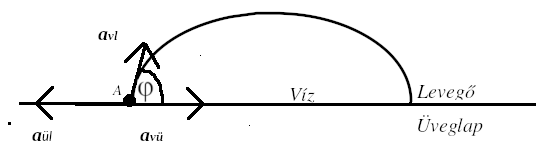
\includegraphics[width=0.7\textwidth]{tetel72.png}
		\caption{Az üveglapon lévő vízcsepp, rajta A egyensúlyban lévő ponttal és a rá ható erőkkel \label{fig:illeszkedesi_szog}}
	\end{center}
\end{figure}

\section{Görbített határfelület}

\footnotesize
\paragraph{Demonstráció} Egy \textit{y} alakú cső mindhárom vége lyukas. Az \textit{y} tején lévő végeit a csőnek szappanos vízzel bevonjuk, majd az \textit{y} szárába levegőt fújunk, majd a szárát befogjuk, hogy levegő nem mehessen se ki, se be. Ekkor az \textit{y} két szárán két buborék lesz, közel azonos mérettel. Az idő múlásával azonban az egyik leeresztődik, a másik pedig nagyobbra fújódik úgy, hogy a két buborék össztérfogata nagyjából állandó. Mi áll a jelenség mögött?
\normalsize

Tekintsük egy kicsiny görbült felületet, amelyet 4 oldalvonal, $\Delta {s_1}$, $\Delta {s_2}$, $\Delta {s_1}$ és $\Delta {s_2}$, továbbá egy belső és egy külső oldal határol. Ekkor az oldalai a felületnek egy körívvel közelíthetőek, $\Delta {s_1}$ mentén $R_1$, $\Delta {s_2}$ mentén $R_2$ görbületi sugárral\footnote{$R_1$ és $R_2$ kellően simán görbülő felületekre mindig egyértelműen meghatározható, gömbre pedig a felület mentén állandó és értéke a gömb sugara.}. A hártya ekkor egy vékony ellipszoidhéjjal van közelítve. Legyen a felület egyensúlyban!

\begin{figure}[htbp]
	\begin{center}
		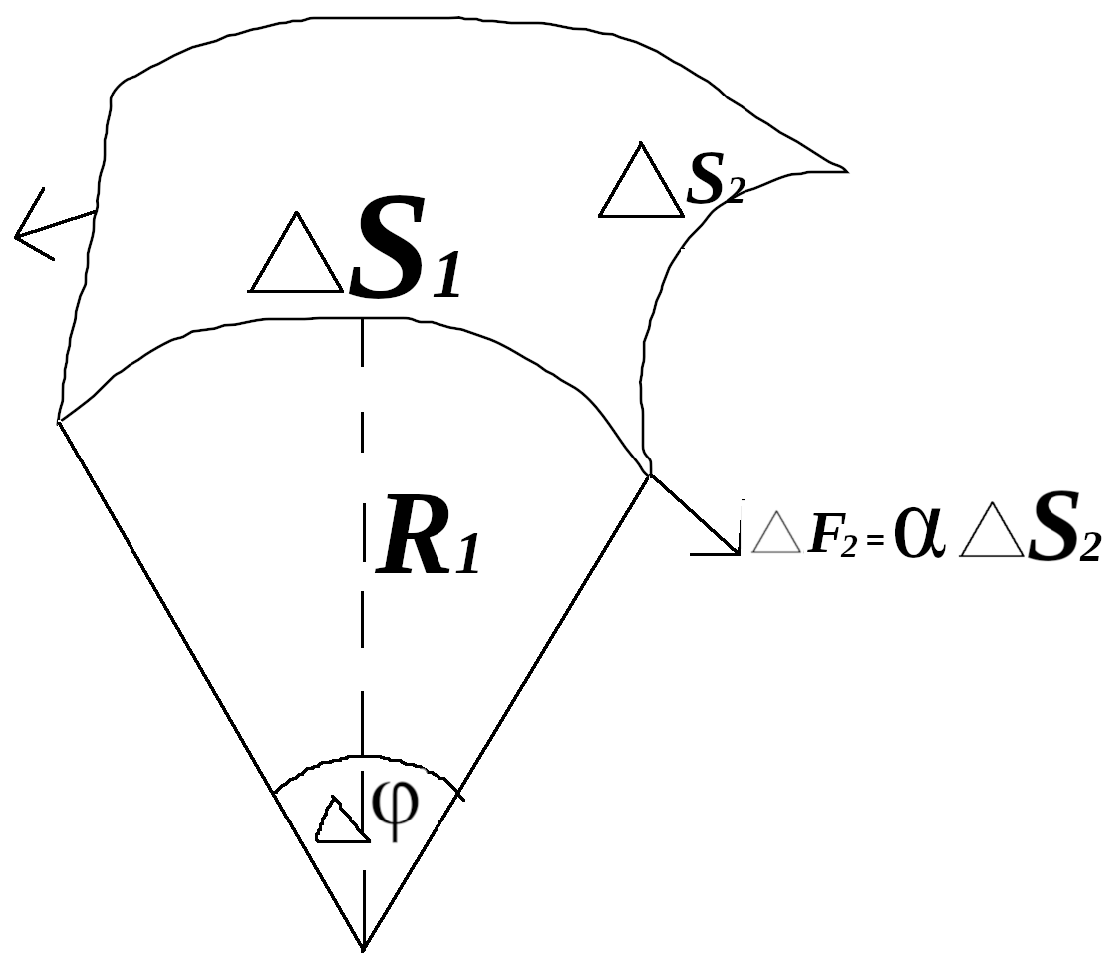
\includegraphics[width=0.4\textwidth]{tetel73.png}
		\caption{Egy kifeszített $\alpha$ felületi feszültségű görbe hártya. }
	\end{center}
\end{figure}

\[\begin{aligned}
  \Delta F =  & \Delta {F_2} &  &  + \Delta {F_1} \\ 
   =  & 2 \cdot \alpha \Delta {s_2}\sin \left( {\Delta {\phi _{\Delta {s_1}}}/2} \right) &  &  + 2 \cdot \alpha \Delta {s_1}\sin \left( {\Delta {\phi _{\Delta {s_2}}}/2} \right)\quad \sin \left( x \right) \to x \\ 
   =  & 2\alpha \Delta {s_2}\frac{{\Delta {s_1}}}{{2{R_1}}} &  &  + 2\alpha \Delta {s_1}\frac{{\Delta {s_2}}}{{2{R_2}}} \\ 
   =  & \Delta {s_2}\Delta {s_1} \cdot \underbrace {\alpha \left( {\frac{1}{{{R_1}}} + \frac{1}{{{R_2}}}} \right)}_{{p_g}} \\ 
   =  & \Delta A \cdot {p_g} \\ 
\end{aligned} \]

Itt már bevezetésre került a $p_g$ görbület nyomás, amit a 
\[{p_g} = \alpha \left( {\frac{1}{{{R_1}}} + \frac{1}{{{R_2}}}} \right)\]
összefüggésből számolhatunk. Ebből is látszik, hogy kisebb sugarú gömb esetén a gömbfelületi nyomás nagyobb, ezért fújja fel a kisebb buborék a nagyobbat. Ha egy buborék egyensúlyban van, akkor a belső oldalán a nyomás a görbületi nyomással lesz nagyobb, mint kívül. Felírva a nyomást a sugár függvényében, a nyomásnak a gömbhéj mentén $p_g$ ugrása van (csökken).

Ezzel a levezetéssel ekvivalens, ha felírjuk a felületi energiát, és megvizsgáljuk, hogyan változik az energia, ha megváltozik a térfogat.
\footnotesize
\paragraph{Storytime}
Ez a jelenség nem csak szappanhártyáknál jelentkezik, hanem minden anyagnál, ahol a határfelület léte magasabb energiaszintet képvisel. Továbbra is a szén és vas példánál maradva, az acélban jelen lévő szén kiválások közötti is hasonló folyamat mehet végbe. Ha olyan a hőmérséklete az ötvözetnek, hogy benne az szén atomok könnyen eldiffundálhatnak egyik helyről a másikra, és az ötvözetben különböző méretű kiválások vannak, akkor a kisebb szén-kiválásokból átdiffundálnak a szén atomok a nagyobb kiválásokba, mert ez csökkenti a felületi energiát. A folyamat mikroszkóppal nyomon követhető, jellemző időskálája a hőmérséklettől függ, de kb.\ órás nagyságrendű, és a sebességéből lehet következtetni a határfelület energiájára. A folyamat neve Ostwald-érés.

Szilárd anyagokban a leíráshoz azt használjuk fel, hogy felírjuk a felületre ható erőket, amelyeket a felület külső oldalán $\sigma_1$, a belső oldalán $\sigma_2$ kelt. Ezek a kicsiny erők tartalmaznak nyírókomponenst, de a felületre merőleges erők eredője
\[\Delta {{\mathbf{F}}_{ \bot ,1}} + \Delta {{\mathbf{F}}_{ \bot ,2}} = {\mathbf{n}}{\hat \sigma _1}{\mathbf{n}} \cdot \Delta A - {\mathbf{n}}{\hat \sigma _2}{\mathbf{n}} \cdot \Delta A = {\mathbf{n}}\left( {{{\hat \sigma }_1} - {{\hat \sigma }_2}} \right){\mathbf{n}} \cdot \Delta A = \alpha \left( {\frac{1}{{{R_1}}} + \frac{1}{{{R_2}}}} \right) \ne 0.\]
Ha $\hat \sigma$ diagonális, akkor a megjelenő diád a nyomás, de általánosan, szilárd testekre $\hat \sigma$ nem diagonális.
\normalsize

\section{Kapilláris emelkedés}

\footnotesize
\paragraph{Demonstráció}
Egy kádba két, mindkét végén nyitott üvegcsövet teszünk. Egy ujjnyi vastagot és egy hajszálvékony üregűt. Azt láthatjuk, hogy a vékony csőben a folyadék szintje magasabb, mint a vastagabb csőben.

Ha megismételjük a kísérletet higannyal, akkor ennek ellenkezőjét láthatjuk. A vékony csőben a higanyszál alacsonyabban van, mint a vastag csőben.

Mi okozza ezt a jelenséget?
\normalsize

\begin{figure}[htbp]
	\begin{center}
		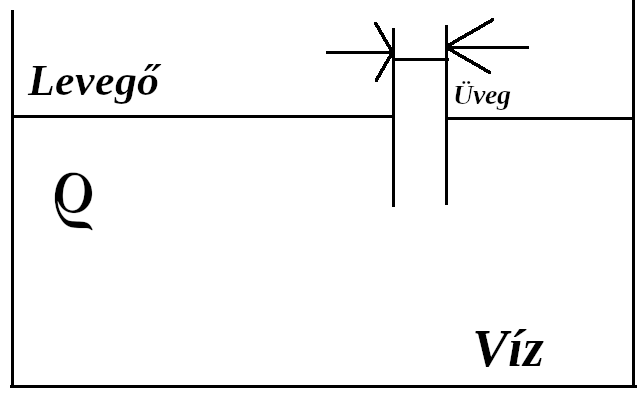
\includegraphics[width=0.3\textwidth]{tetel74.png}
		\caption{A vízbe merített kapilláris csőben a víz magasabban áll, mint az edényben.}
	\end{center}
\end{figure}

Írjuk fel az energiáját a vízoszlopnak, ami a víz felszíne felett van! Ez származik egyrészt a potenciális energiájából, a víz-üveg felületi energiából, illetve az elveszített levegő-üveg felületi energiából,
\[E\left( h \right) = {r^2}\pi h\varrho g\frac{h}{2} + 2r\pi h{\alpha _{{\text{ü,v}}}} - 2r\pi h{\alpha _{{\text{ü,l}}}},\]
ahol $h/2$ a tömegközéppont emelkedése. Ez akkor lesz egyensúlyban, ha a $E\left( h \right)$ függvénynek minimuma van, azaz
\[\frac{{dE\left( h \right)}}{{dh}} = 0 = {r^2}\pi h\varrho g + 2r\pi \left( {{\alpha _{{\text{ü,v}}}} - {\alpha _{{\text{ü,l}}}}} \right).\] 
Ebből
\begin{equation} \label{eq:kapillaris_emelkedes}
h = \frac{{2}}{{r \varrho g}}\left( {{\alpha _{{\text{ü,l}}}} - {\alpha _{{\text{ü,v}}}}} \right).
\end{equation}
Ez az összefüggés megmutatja, hogy minél vékonyabb a cső, a folyadék emelkedése annál nagyobb. A jelenség neve kapilláris emelkedés. Az $\alpha$ felületi feszültség értéke nélkül nem tudható, hogy milyen méretskálán látható a jelenség, de a konkrét anyagi minőség mellett, azaz víz, üveg és levegő esetén a milliméter alatti skálán figyelhető meg jól a kapilláris emelkedés. Higany esetére a számok viszonyai fordítottak, az argumentumban negatív érték van, így a $h$ emelkedési magasságra negatív értéket kapunk.
\footnotesize
\paragraph{Storytime} Ha a kapilláris mérete a sejtek nagyságrendjébe esik, mint pl.\ a fánál, akkor az emelkedés mértéke több méter is lehet. Hasznos ez a jelenség még a vízvezeték csövek szerelésénél is, amikor a vizet szállító réz csöveket illesztenek össze. Az illesztésnél az egyik rézcső átmérője kisebb, mint a hozzá toldotté, és a két cső egymásba csúsztatható, de ettől még nem zár tökéletesen a vízzel szemben, mi több, a csőben a légköri nyomást akár néhányszor meghaladó nyomás is lehet. A két cső közötti kis részt forrasztóónnnal hézagolják ki. Ehhez felmelegítik a két csövet a forrasztóón olvadási hőmérséklete fölé (megfelelő ötvözetek használatával $230{,}^\circ$C-tól felfelé, folytonosan állítható olvadásponttal). A megolvadt forrasztóón pedig a két cső közötti vékony rétegbe a kapilláris emelkedés jelensége segítségével bejut és tökéletesen zárja a vizet nyomás ellenében is. A technológiát kapilláris forrasztásnak nevezik.

Hasonló a jelenség a kerámia anyagoknál is, pl.\ párologtatókkal is. A kiégetett kerámiában kapilláris hálózatok vannak, így a mázatlan kerámiára cseppentett víz az egész kerámiában szét tud terjedni, lefele és felfele is. A tárcsafékek kerámia fém betétei pedig éppen ezért érzékenyek az olajokra, amelyek a fékhatást gyengítik. A fékbetétre jutó olaj a kapillárisrendszerben könnyen szétterül és tárolódik, ezért hiába tisztítják le a féktárcsa és fékbetét felületét az olajos szennyeződések eltávolításáért, a kerámia betétben az olaj benne marad, és fékezésnél apránként újra bekeni a féktárcsát.
\normalsize

\subsection{Illeszkedési szög}
A folyadék felszínét vízszintessel közelíteni nem rossz feltételezés, ha a csőben tárolt folyadék mennyiségét adjuk meg. Azonban a csövet nagy nagyításban nézve látható, hogy annak felülete ívelt, mert van egy illeszkedési szög a hármas határfelületen, mint ahogy azt \aref{fig:illeszkedesi_szog}.\ ábrán láthattuk, amit a \aref{fig:kapillaris_illeszkedesi_szog}.\ ábra szemléltet.

\begin{figure}[htb]
	\begin{center}
		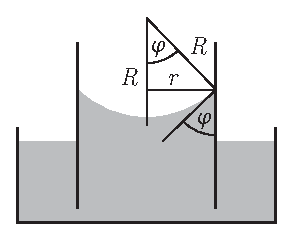
\includegraphics[scale=1]{kapillaris_emelkedes_illeszkedesi_szog.eps}
		\caption{A kapillárisban a vízfelszín ívelt, $R$ görbületi sugárral. }
		\label{fig:kapillaris_illeszkedesi_szog}
	\end{center}
\end{figure}
\FloatBarrier

Ebben az esetben a határfelület egyensúlyára azt írhatjuk fel, hogy a kerületre ható, felületi feszültségből származó erő a gravitációs erőnek tart ellen. Ezzel a megfontolással \az{\eqref{eq:kapillaris_emelkedes}}.\ egyenlet szintén megkapható, illetve a $\varphi  = \arccos \left( {r/R} \right)$ illeszkedés szöggel kifejezve (amelyre fennáll \az{\eqref{eq:illeszkedesi_szog}}.\ egyenlet)
\begin{equation}
\left. \begin{gathered}
  h = \frac{2}{{r\varrho g}}\left( {{\alpha _{{\text{ü,l}}}} - {\alpha _{{\text{ü,v}}}}} \right) \hfill \\
  \cos {\left( \varphi  \right)}  = \frac{{{\alpha _{{\text{l,ü }}}} - {\alpha _{{\text{ü,v}}}}}}{{{\alpha _{{\text{v,l}}}}}} \hfill \\ 
\end{gathered}  \right\}h = 2\frac{{{\alpha _{{\text{v,l}}}}\cos \left( \varphi  \right)}}{{\varrho gr}} = 2\frac{{{\alpha _{{\text{v,l}}}}}}{{\varrho gR}}.
\end{equation}



\section{Felületek tulajdonságai}
Mint láthattuk, a megjelenő felületek egy új fizikát hoznak be, amelyek nem írhatóak le a térfogati tulajdonságokkal, azok mellett új empirikus jelenségként kezelhetőek. Valójában persze mind a térfogati, mind a felületi tulajdonságok kiszámolhatóak a mikroszkopikus, atomi szintű viselkedésekből, de ezek kvantitatív kiszámolása túl időigényes és bonyolult, ellenben könnyen leírhatóak makroszkopikus szinten, kontinuum közelítésben, ahol a térfogati és felületi tulajdonságokat különválasztva írjuk le.
\end{document}